\documentclass[letterpaper,twocolumn,10pt]{article}

% Use draftpaper for notes and date markings on every page.  Useful when you
%   have multiple copies floating around.
% Use offcenter for the extra .5 inch on the left side. Needed with fullpage and fancy.
% Use mixcasechap for compatibility with hyperref package, which does NOT like all caps default
% Use edeposit for the adviser/committee on the title page.
% Use tocnosub to suppress subsection and lower entries in the TOC.
% PhD candidates use "proquest" for the proquest abstract.

\makeatletter

\usepackage{setspace}
\usepackage{epsfig}  % for figures
\usepackage{amsmath}  % for math spacing \usepackage{lscape}  % Useful for wide tables or figures.
\usepackage{algorithm}
\usepackage{algpseudocode}
\usepackage{color}
\usepackage{xcolor}
\usepackage{xspace}
\usepackage[justification=raggedright]{caption}	% makes captions ragged right - thanks to Bryce Lobdell
\usepackage[hyperfootnotes=false]{hyperref}

\hypersetup {
    citebordercolor=green,
    bookmarks=true,
    linktoc=all
}

\begin{document}

\date{}

\title{\Large \bf User-Guided Meta-Path Based Framework for Heterogeneous Networks}
\author{
    {\rm Hilfi Madari Alkaff, Efe Karakus}\\
    \{alkaff2, karakus1\}@illinois.edu
}

\maketitle
\thispagestyle{empty}

\subsection*{Abstract}

With the advent of the big-data era, there have been many large-scale
heterogeneous information network that consist of multi-typed, interconnected
objects such as social media networks or news networks. Many companies have
been established to unearth patterns in such a massive dataset. One of the
operations that people have been interested is performing is similarity search.
However, most existing similarity search frameworks have been unable to support
user queries in real-time. Furthermore, users are not able to perform OLAP
operations efficiently on the data. As a result, it is not possible for user to
compute similarity measures between two objects under the contexts that the
user desires. In this paper, we propose similarity search that support both
online and OLAP queries for user.

\section{Introduction}
\label{sec:introduction}

In the current era of big data, an enormous amount of information is being
generated in real-time. It is important that we are able to navigate these
massive datasets to understand what is currently going on. We would like to
specifically focus on news data for a number of reasons. Firstly, there is an
abundance of available news data that we could analyze. Secondly, it is
possible to categorize news data hierarchically. An example of such hierarchy
is the country, followed by state, district, and so on. We should be able to
seamlessly navigate between different level in the hierarchy to retrieve the
relevant information. Last but not least we choose news data because it allows
us to be more aware of the current events that are happening around us. As
such, we would like a platform that allow us to answer questions such as 'Who
are the key politicians for healthcare reforms?', 'How did the opinion of
Barack Obama change over time for education?' and so on.

Similarity search has been extensively studied in the past. At first, it was
applied to only categorical and numerical data types in relational data. Then,
there have been works that tries to leverage link information in networks. Most
of these studies focus on homogeneous or bipartite
networks~\cite{page1999pagerank, jeh2002simrank, xu2007scan}. However,
these similarity measures disregard the subtlety of different types among objects and links
which are present in heterogeneous information network. More recently, a
meta-path based similarity framework, PathSim~\cite{sun2011pathsim}, has been proposed
that takes into account different linkage in the network.

However, there are several shortcomings in the PathSim design.
Firstly, the operations to compute the meta-path are computationally expensive
and consume a lot of memories since it is achieved through matrix multiplications.
Secondly, it does not allow users to perform any OLAP operations in the dataset.
This is important because a user might be interested in the similarity of two
objects under a specified context only. Thirdly, the original PathSim framework
also does not allow user to provide hints in the type of meta-paths that a similarity
search query should return. For instance, a user might be interested in a similarity
search between two objects that does not go into a specific node in the graph.

In this paper, we propose \h, which is built on top of PathSim, that addresses
the aforementioned shortcomings of PathSim. We address the first challenge
by building a hash-table, \mTable, whose key is a pair of node while the value is
the meta-paths between the pair. At first, the hash-table is empty. But as
user queries for similarity measures on two nodes in the graph, the meta-paths
found during the computation will be cached in the hash-table. This
allows for faster indexing if the user performs the same query. For the
second challenge, we address it by (TALK ABOUT FOREST.PY). Finally,
the third challenge is addressed by keeping track of constraints that
the user specifies in a hash-table, \cTable. \cTable will be
checked whenever we found a candidate for meta-path between two objects
to ensure that none of the constraints that the user specified is
violated.

\subsection{Paper Outline}

This paper is structured as follows. We begin with the design of our framework
(Section~\ref{sec:design}) followed by our implementation
(Section~\ref{sec:impl}). We then show our the performance of our framework
based on the DBLP and NYTimes dataset (Section~\ref{sec:eval}). Following that,
we will then survey related works in the area (Section~\ref{sec:rel-work}).
Finally, we discuss some extensions that could further be made to our framework
and conclude (Section~\ref{sec:conc}).

\section{Design}
\label{sec:design}

In this section, we begin with describing PathSim framework in greated detail.
Then, we will delve into the changes that we made to the PathSim framework to
implement a more efficient similarity search framework while being able to
support hints and OLAP operations from the user.

\subsection{PathSim}

PathSim is developed to compute
similarity measures in a heterogeneous information network which are logical
networks that involve multiple typed vertices and multiple typed links denoting
different relations (e.g., bibliographic network, news articles).

Figure~\ref{fig:relationship} shows an example heterogeneous information
network.  In this figure, there are 4 possible types of entities, author,
paper, venue and term, which are inter-connected while there are also 4
different type of edges that exist (i.e., ''Writes``, ''Has``, ''Cited`` and
''Submitted To``).

\begin{figure}[H]
    \centering
    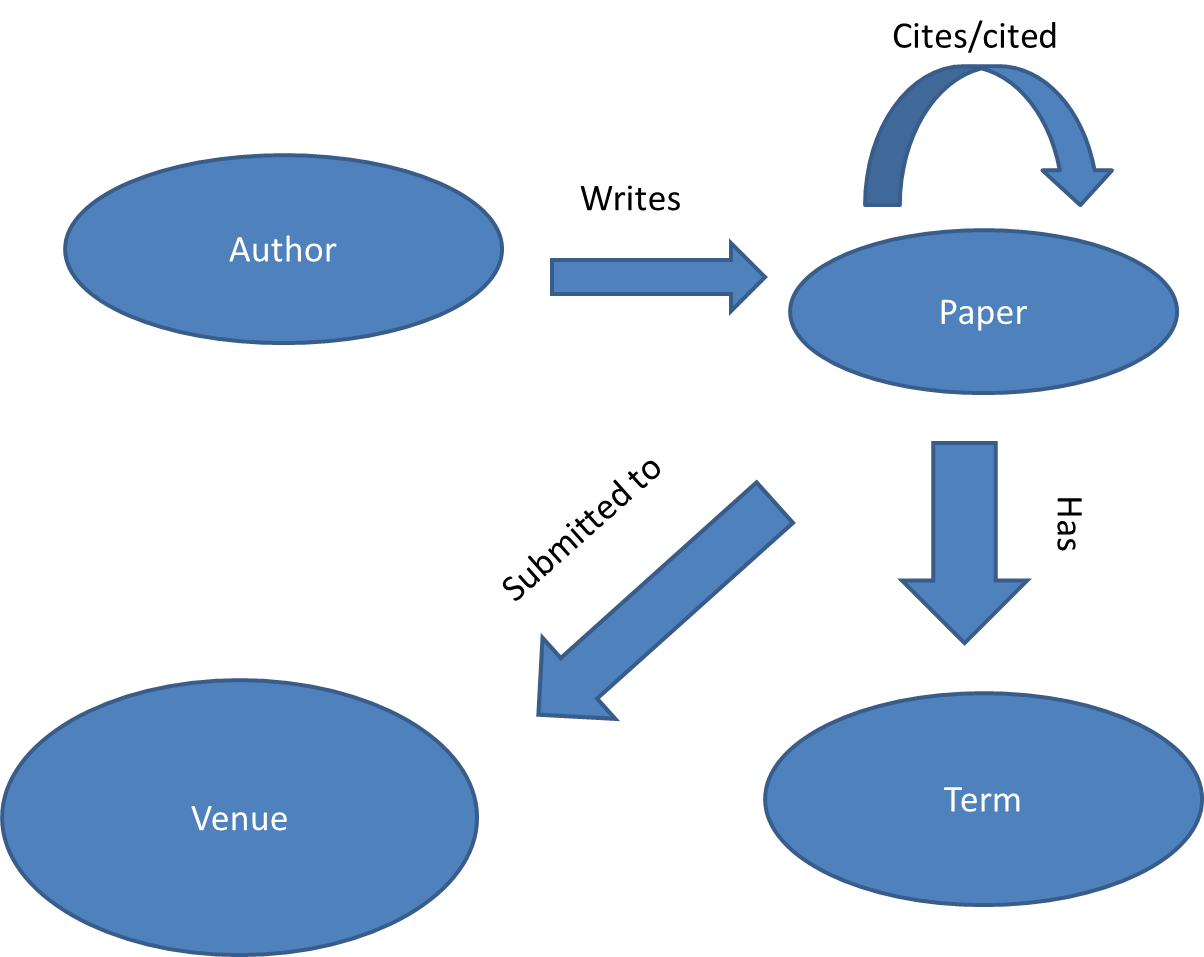
\includegraphics[width=0.6\linewidth]{./figs/relationship.png}
    \caption{Bibliographic Network}
    \label{fig:relationship}
\end{figure}

PathSim strives to define similarity measures between vertices in heterogeneous
information network using structural information and to answer top-k similarity
search queries efficiently. It accomplishes this by developing a novel meta
path-based framework.

As shown in Figure~\ref{fig:relationship}, entities can be connected via
different connectivity paths. For instance, two authors can be connected via
author-paper-author (i.e. co-authors) path or author-paper-venue-paper-author
(i.e.  the authors submitted both of their papers to the same conferences)
path. Intuitively, the different paths represent a different similarity
semantics. More formally, as written in the paper, the meta path can be
described as follows:

\begin{Def}
\label{meta path}
\textbf{Meta path}. A meta path $\mathcal{P}$ is a path defined on the graph on
network schema $\mathcal{T_G} = \mathcal{(A, R)}$, and is denoted in the form
of $\mathcal{A}_1 \xrightarrow{R_1} \mathcal{A}_2 \xrightarrow{R_2} \cdots
\xrightarrow{R_l} \mathcal{A}_{l + 1}$ which defines a composite relation
$\mathcal{R} = \mathcal{R}_1 \circ \mathcal{R}_2 \circ \cdots \circ
\mathcal{R}_l$ where $\circ$ denotes the composition operator on relations. \newline
\end{Def}

Although multiple similarities measure have been previously explored such as
path counting or random walk-based similarity, they are biased to either
popular entities and thus unable to capture the essence of peer similarity.
For instance, if we would like to find out about authors that are similar to
an early PhD student that has published a few papers, the above measures
will yield professors who happen to co-author with this particular student
although what we desire are other PhD students. This has become the other
motivation for PathSim. Using the concept of meta path above, Path-Sim
defines the relationship between two entities as follow: \newline

\begin{Def}
\label{path-sim}
\textbf{PathSim: A Meta path-based similarity measure}. Given a symmetric
meta path $\mathcal{P}$, PathSim between two vertices of the same type
x and y is:

\begin{align*}
s(x,y)=\frac{2*|\{p_{x \rightsquigarrow x}:p_{x \rightsquigarrow y}\}|\in\mathcal{P}}
{|\{p_{x \rightsquigarrow x}:p_{x \rightsquigarrow x}\}|\in\mathcal{P} +
|\{p_{y \rightsquigarrow y}:p_{y \rightsquigarrow y}\}|\in\mathcal{P}}
\end{align*}

where $p_{a \rightsquigarrow b}$ is the meta paths between $a$ and $b$. \newline
\end{Def}

Intuitively, this indicates that if $x$ is popular, but not $y$, the number of
meta paths between $x$ and itself will be much larger than the number of
meta paths between $x$ and $y$. Thus, when we are comparing a popular entity
and an un-popular entity $s(x,y)$ will be low and vice versa. We need to have
either both to be popular or un-popular so that $s(x,y)$ yield a considerable
value.

\subsection{hPathSim}

There are three main improvements that we made to the PathSim framework.
Firstly, even with the pruning algorithm that they introduce in the paper,
the original PathSim framework still requires expensive matrix computations
that are not feasible in an online setting. We introduce a better storage
mechanism, \mTable, that allows faster materialization of the meta paths. Secondly,
we built our own tree data structure, \hTable, to allow us to perform
efficient OLAP operations on the dataset. Thirdly, we show how we are able
to support user defined constraints in our dataset.

% Depending on the meta path that it wants to materialize

\subsubsection{Storage Optimization}

In \h, we introduce a hash-table in which the key is a pair of node,
$(\mathcal{N}_1, \mathcal{N}_2)$ while the value is a set of meta paths between
the pair.  At first, the hash-table is empty. But as user queries for
similarity measures on two vertices in the graph, meta-paths found during the
computation will be cached in the hash-table. This enables fast retrieval if
the user issues the same queries in the future.

However, as noted in the original PathSim paper, it is impossible to cache all
of the possible meta-paths in an enormous graph. The author of the paper
calculated the storage size requirement of all the possible length-4 meta paths
in the DBLP data set is more than 40GB. Thus, we use an underlying database in
our framework to regularly swap meta paths in the cache to the disk if we are
using too much memory. We use Least Recently Used (LRU) policy to determine
which meta paths that need to be swapped to the disk due to its simplicity and
its effectiveness in ensuring that it works.

The database is checked every time the user issues a similarity search query to
see if meta paths between two vertices have been computed previously. If so, the
meta paths will be swapped back to the cache again. Similar to our cache, the
database will still be indexed by $(\mathcal{N}_1, \mathcal{N}_2)$ to allow
fast retrieval.

\subsubsection{Hierarchy Forest}

The heterogeneous network contains hierarchies for certain entities. For example,
a location hierarchy could look like:

\begin{align*}
Urbana \leadsto USA \leadsto North America \leadsto root
\end{align*}

\h builds a forest of hierarchical trees, the trees are using HashTables in their core to
allow for fast lookup of a node in the tree. The roll-up and drill-down operations
on the tree are implemented just by using a depth-first search (DFS).

The forest provides 5 key operations for each of the trees:
\begin{itemize}
    \item \textit{is\_member(nodeTitle, queryID)}: Applies an iterative DFS to check if
    the node with id \textit{queryID} is under the subtree of \textit{nodeTitle}.
    \item \textit{is\_slice(nodeTitle, queryID)}: check whether the node with $nodeTitle$
    has the id $queryID$.
    \item \textit{get\_categories()}: return the tree titles in the forest.
    \item \textit{get\_children(nodeTitle)}: get all immediate children under the node
    $nodeTitle$.
    \item \textit{get\_parent(nodeTitle)}: get the parent of the node $nodeTitle$.
\end{itemize}

All the operations described above take $O(1)$ run-time due to the HashTable, except for
\textit{is\_member} which can take $O(N)$ where $N$ is the number of nodes under the specified
hierarchy tree.

\subsubsection{User-Specified Constraints}

Thirdly, we also allow user to specify constraints on the type of meta paths
result that are used for computing the similarity score. There are two types of
constraints that the user could specify. Firstly, a user could specify that
meta paths between two vertices must go through a certain node or any nodes
with a particular category type. Conversely,  a user could also specify that
meta paths between two vertices must not go through a certain node or any nodes
with a particular category type. We choose these two types of constraints
becaues we believe that they are intuitive for the users and will allow users
to identify similarity between the two objects in a greater detail. These
constraints are stored in a hash-table, \cTable.

Similar to the original PathSim framework, the top-k paths used for the
similarity search computation are discovered through a Breadth-First Search
(BFS) algorithm. We based our algorithm off BFS due to its simplicity and guarantee to
compute shortest path between two vertices. The first constraint is being
enforced as we add a node into our candidate set

\begin{algorithm}
    \caption{Constrained BFS Algorithm to Find Meta-Paths}
    \label{alg:1}
    \begin{algorithmic}[1]
        \Function{FindPath}{c, src, dst}
            \State q $\gets$ Queue()
            \State paths $\gets$ Set()
            \State q.enqueue(Array(src))
            \State
            \While {not q.empty()}
                \State curPath $\gets$ q.dequeue()
                \State lastNode $\gets$ curPath.lastNode
                \For {n $\leftarrow$ lastNode.neighbors}
                    \If{checkConstraint(n, c, "mustNotHave")}
                        \State continue
                    \ElsIf{n in curPath}
                        \State continue
                    \EndIf
                    \State

                    \State newPath $\gets$ curPath.append(n)

                    \If{n $==$ dst}
                        \If{checkConstraint(n, c, "mustHave")}
                            \State paths.add(newPath)
                        \EndIf
                    \Else
                        \State q.enqueue(newPath)
                    \EndIf
                \EndFor
            \EndWhile
            \State
            \State \Return{paths}
        \EndFunction
    \end{algorithmic}
\end{algorithm}

Algorithm~\ref{alg:1} shows the algorithm that we use to discover the top-k
paths with user-specified constraints. The first $checkConstraint$ function
is called every time a new partial path is explored. It ensures that nodes
that user \textit{does not want} to be added are being pruned from the search
space to save computation time. The second $checkConstraint$ function
is called only when a full candidate path between the source and destination
is discovered. This ensures that all the nodes that the user \textit{wants}
exist in the path.

\section{Evaluation}
\label{sec:eval}

In this section, we begin with describing the datasets used in our experiments
before evaluating the performance of \h on those datasets.

\subsection{Datasets}

We test \h on two different datasets.

% The DBLP dataset is a network of Authors, Papers, Citations, Venues, and
% Terms. It is a heterogeneous network, however it does not contain any
% hierarchical entities. The total size of the data is 1.1GB, the relationship
% between entities were as follow: Author$\leftrightarrow$Paper,
% Paper$\leftrightarrow$Term, and Paper$\leftrightarrow$Venue.

The DBLP Hierarchical Dataset is similar to the previous one. Except, that now
the relations are as follows: Paper$\leftrightarrow$Area,
Author$\leftrightarrow$Area, Conf$\leftrightarrow$Area,
Term$\leftrightarrow$Area.  Furthermore, Area and Conf entities form a
hierarchy.  This dataset is much more smaller than the previous one, only
7.9MB. There are 70536 vertices in this dataset with each node having
an average degree of 9.0 with a standard deviation of 74.8. The average
path length is 4.0 with a standard deviation of 1.10.

Finally, the last dataset is from the New York Times. It represents a
comprehensive dataset that is both heteregenous and also hierarchical. The
network is 650MB, with entities: Article, Location, Organization, Person,
Topic. Furthermore, each one of these entites except Article has its own
hierarchy. There are 181874 vertices in this dataset with each node having an
average degree of 10.0 and a standard deviation of 73.7. The average path length
is 4 with a standard deviation of 0.97.

\subsection {Experiments}

There are three main metrics that we would like to evaluate the performance of
our \h framework on: the runtimes similarity search query, drill-down and
roll-up OLAP queries. Since the underlying similarity search algorithm used is
the same as PathSim, the accuracy of \h is also the same and thus, we do not
display the comparison.

\begin{table}
    \centering
    \begin{tabular}{| l | l | l |}
        \hline
        Graph & Average (s) & Stddev \\ \hline
        DBLP Full & 5.26 & 0.042 \\ \hline
        NYT Full & 5.12 & 0.157 \\ \hline
        DBLP DB & 1.41 & 0.03 \\ \hline
        NYT Jordan & 1.70 & 0.04 \\
        \hline
    \end{tabular}

    \caption{Average time taken and standard deviation for similarity search on random pairs of entities in the DBLP and NYTimes datasets.}
    \label{tab:similarity-result}
\end{table}

For the similarity search, we measure the times it takes to
execute similarity search on a pair of nodes with meta-path length of 4. The
evaluation was repeated 5 times. Table~\ref{tab:similarity-result} shows
the time taken on 4 graphs. The first two are
the full DBLP dataset and the full NYTimes dataset while
the last two are a subgraph of the DBLP dataset whose
vertices' ''area`` dimension is database and a subgraph of the NYT
datasets whose vertices' ''country`` dimension is Jordan.
We can see that although, we increase the graph size considerably with
NYT Full our runtimes are about the same. We can also see that
the standard deviation for similarity search is low, hence our results
should be stable.

\begin{table}
    \centering
    \begin{tabular}{| l | l | l |}
        \hline
        Graph & Average (s) & Stddev \\ \hline
        DBLP drill down & 0.055 & 0.024 \\ \hline
        DBLP roll up & 0.0058 & 0.00093 \\ \hline
        NYT drill down & 0.52 & 0.06 \\ \hline
        NYT roll up & 19.22 & 0.91 \\
        \hline
    \end{tabular}

    \caption{Average time taken and standard deviation to perform drill-down
    and roll-up on the DBLP and NYT datasets.}
    \label{tab:similarity-time}
\end{table}

For the OLAP operations, we measure the time it takes to
perform drill-down and roll-up under specific categories.
For the DBLP data the drilled-down subgraph is four times smaller
than the original graph. On the other hand, there was no subgraph in NYT 
that would allow us to get a network of size four times smaller. So we resorted to 
a network that was only 10 \% smaller than the original one.
 Table~\ref{tab:similarity-result} shows
the time taken for OLAP operations on both the DBLP and NYTimes dataset.
We can see that the drill-down operations are really performant, however roll-up can
take a long amount of time when we are dealing with a very large network.

\section{Related Work}
\label{sec:rel-work}

\paragraph{Similarity Search:} We built our framework on top of PathSim because
most similarity measures only work for homogeneous network such
as Personalized Page-Rank~\cite{jeh2003scaling}, Sim-Rank~\cite{jeh2002simrank}
and SCAN~\cite{xu2007scan} although many of the emerging information are
heterogeneous in nature.

\section{Conclusion}
\label{sec:conc}

In this paper, we built \h, a similarity search framework, that improves on the
PathSim. Firstly, even with the pruning algorithm that they introduce in the
paper, the original PathSim framework still requires expensive matrix
computations that are not feasible in an online setting. We introduce a better
storage mechanism, \mTable, that allows faster materialization of the meta
paths to support real-time user queries. Secondly, we built our own tree data
structure, \hTable, to allow us to perform efficient OLAP operations on the
dataset. Thirdly, we also allow users to specify constraints on the meta paths
that are used in the similarity measures.

\subsection{Future Work}

For future work, we plan to implement better search algorithm than our current
implementation. A metaheuristic optimization technique such as ant-colony
optimization algorithm~\cite{dorigo1997ant} will be better at navigating the
graph with the constraints that the user added.

Another area of future will be to make our framework more scalable by running
it in a distributed fashion. There have been previous works that implement
distributed graph processing framework such as GraphLab~\cite{low2010graphlab}
and Graphx~\cite{xin2013graphx}.

\subsection{Open Source}

\h is open source and is available for download at
\url{https://github.com/hilfialkaff/newsnet}.


\bibliographystyle{abbrv}
\bibliography{main}

\end{document}
\endinput
